\section{Applicación Movil}
    La aplicación movil fue desarrollada en el lenguaje de 
    programación Dart utilizando el \acrshort{sdk} de código abierto 
    Flutter. 

    \begin{figure}[htp!]
        \centering
        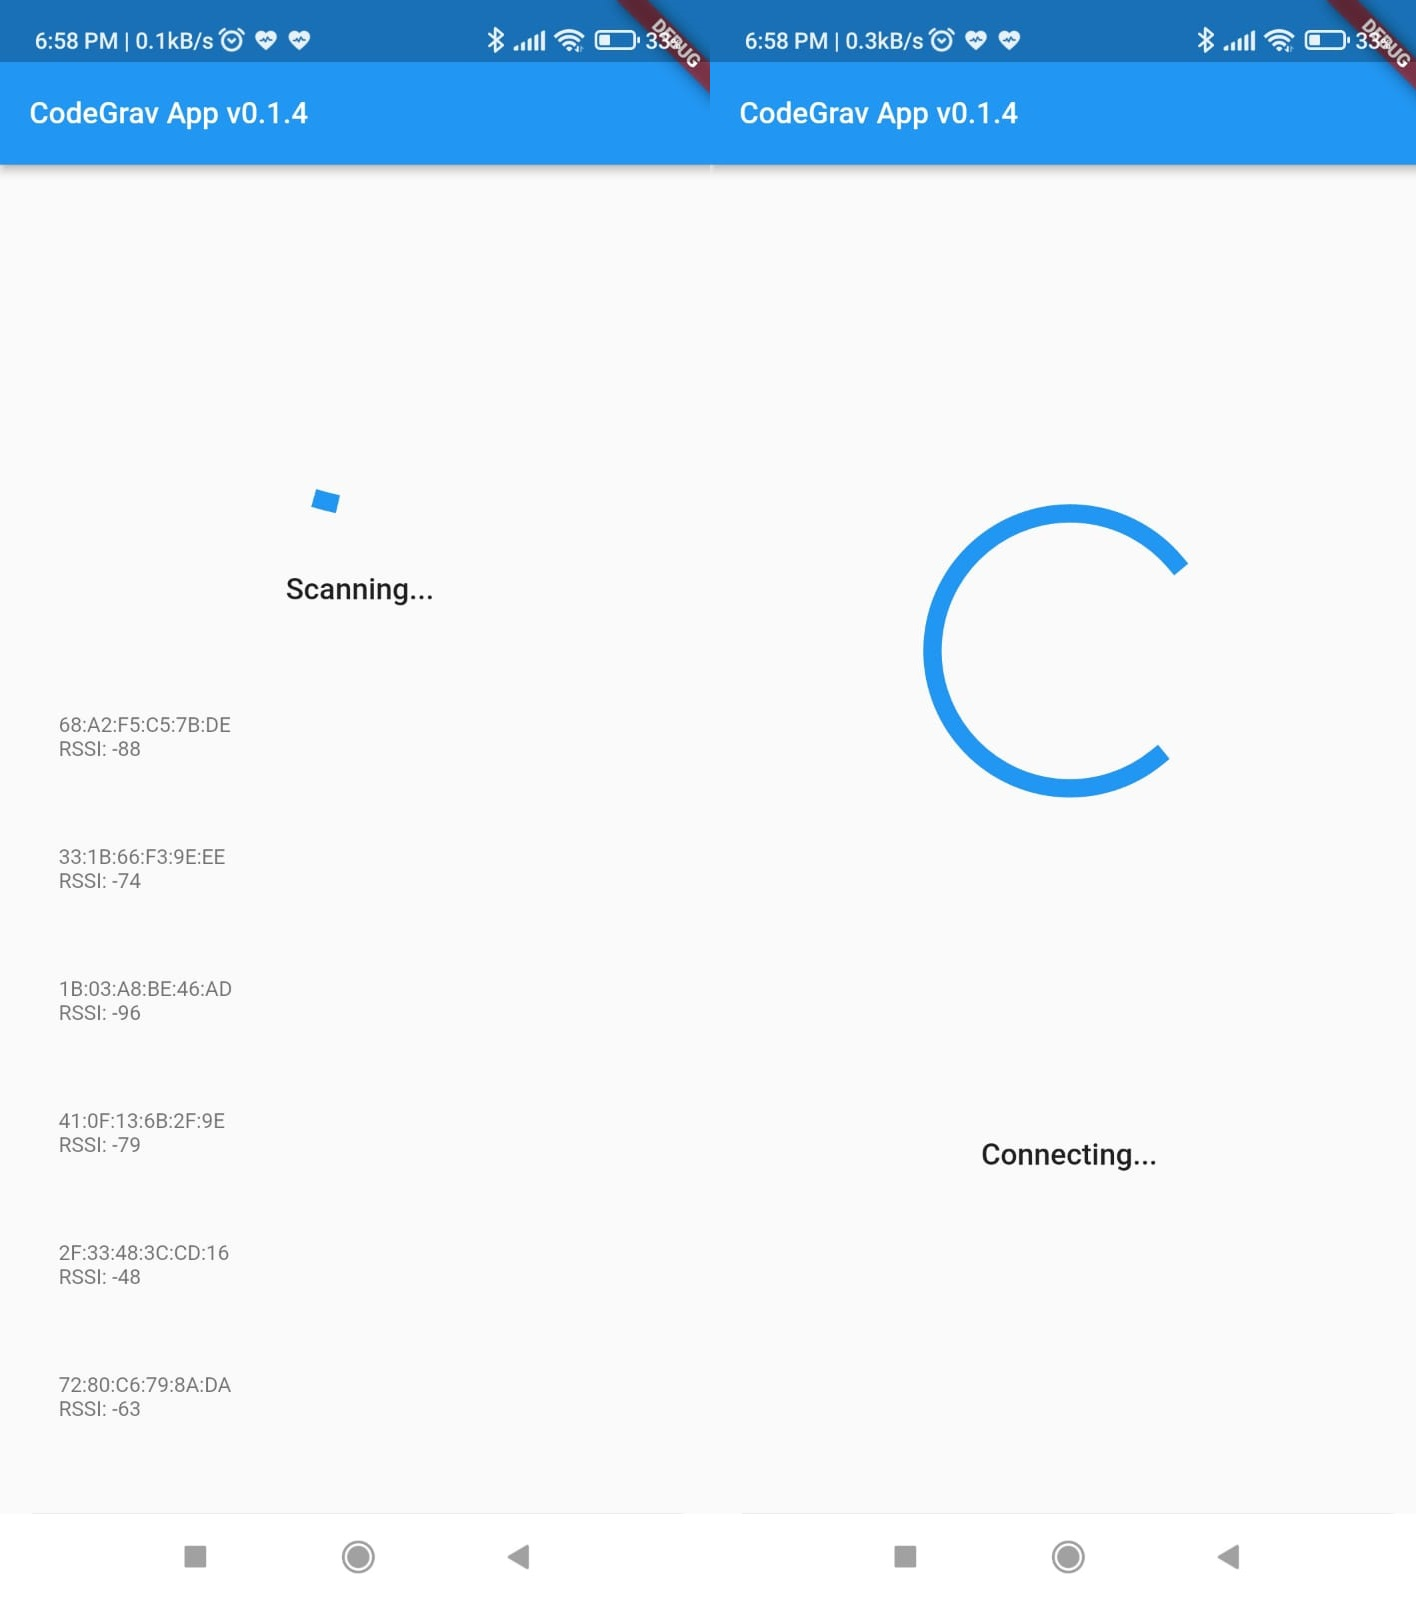
\includegraphics[width = 0.35 \textwidth]{searching_app.jpg}
        \caption{Pantalla de escaneo y conexión.}
        \label{fig: searching_app}
    \end{figure}
    \FloatBarrier

    En la figura \ref{fig: searching_app} se muestra la pantalla de escaneo, en dicha 
    pantalla la aplicacion se queda a la espera de que el dispositivo
    se empareje.

    \begin{figure}[htp!]
        \centering
        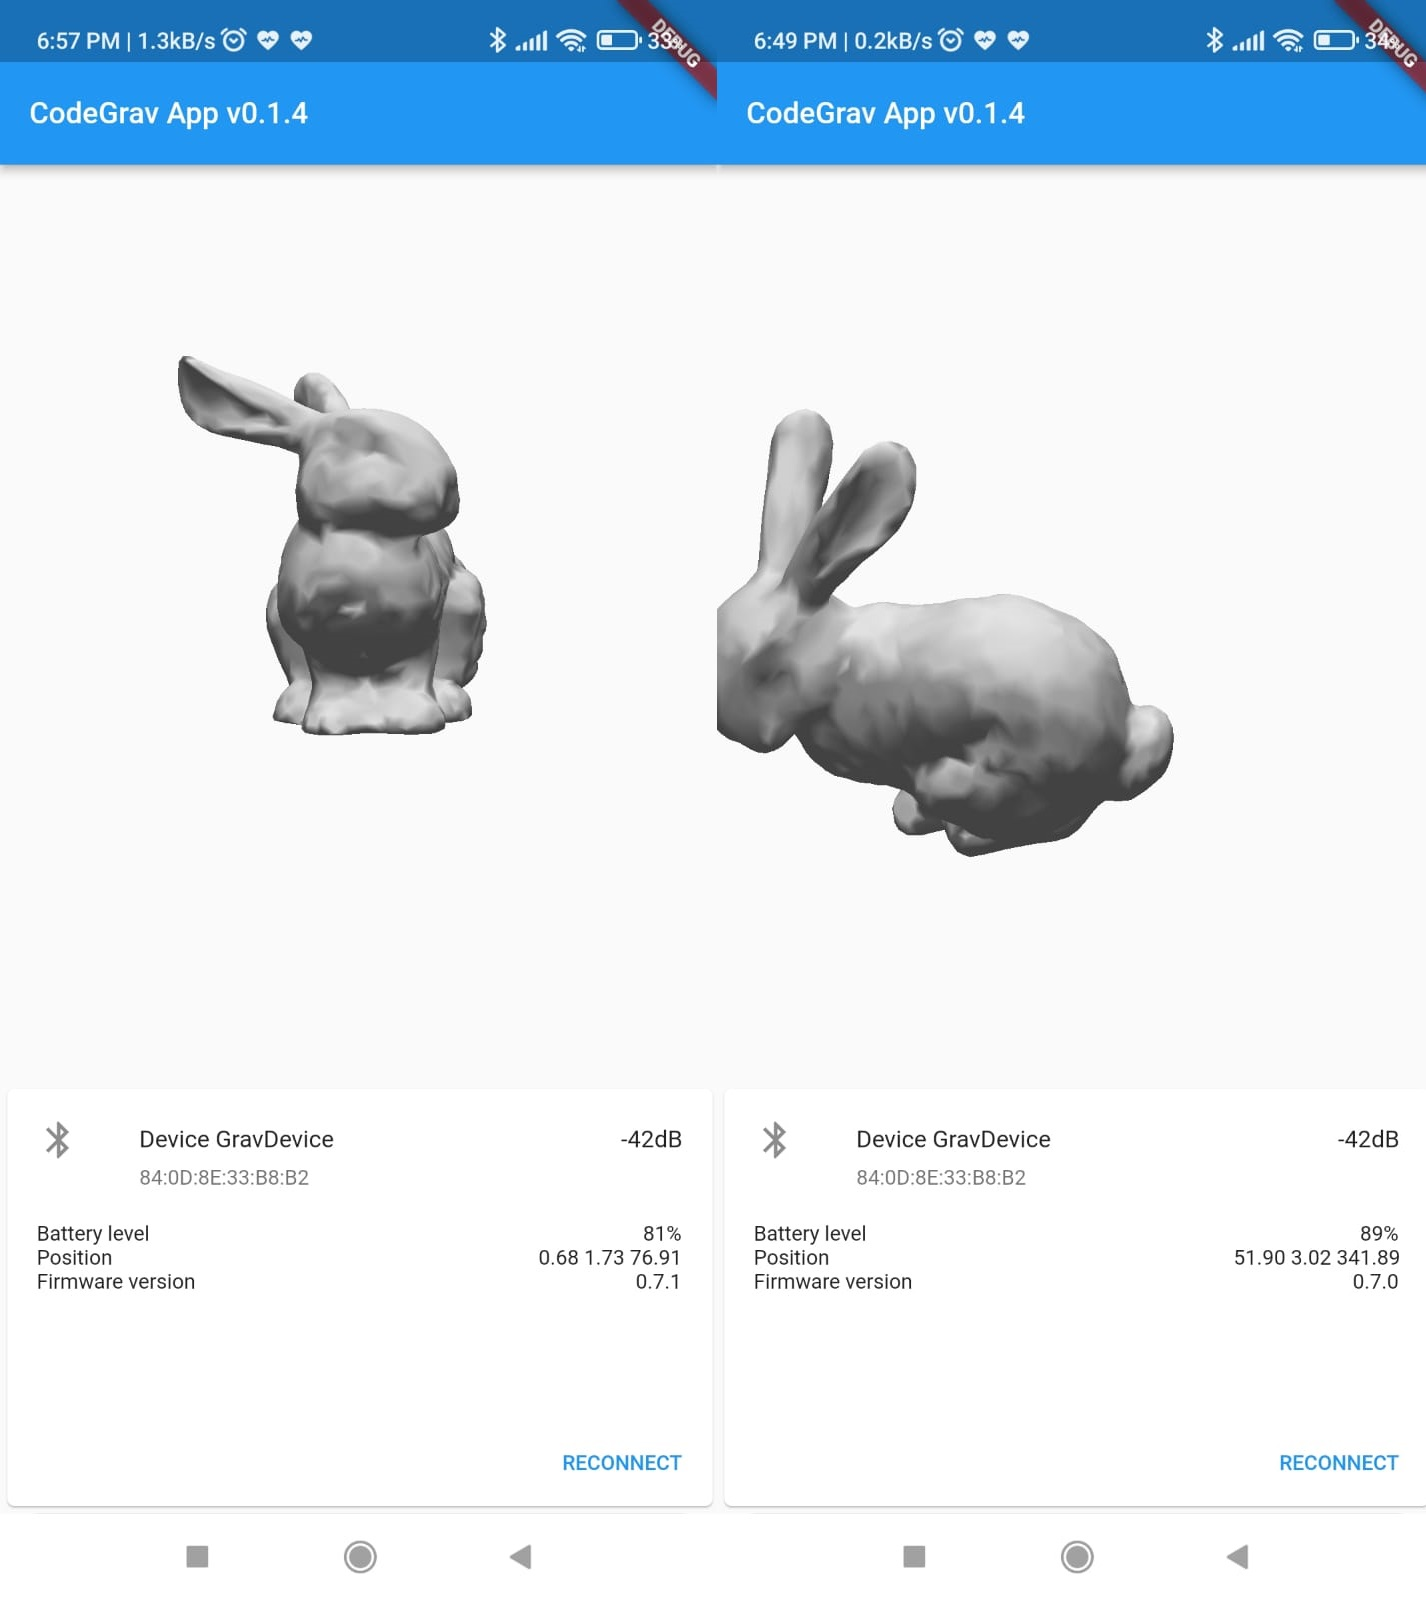
\includegraphics[width = 0.35 \textwidth]{main_app.jpg}
        \caption{Pantalla principal.}
        \label{fig: main_app}
    \end{figure}
    \FloatBarrier

    En la figura \ref{fig: main_app} se muestra la pantalla principal donde disponemos de los
    siguientes elementos: 
        \begin{itemize}
            \item Un modelo 3D que es utilizado para mostrar de forma grafica 
            la orientación del bebe.
            \item La dirección física del dispositivo.
            \item Las mediciones recabadas del disposito.
        
        \begin{figure}[htp!]
            \centering
            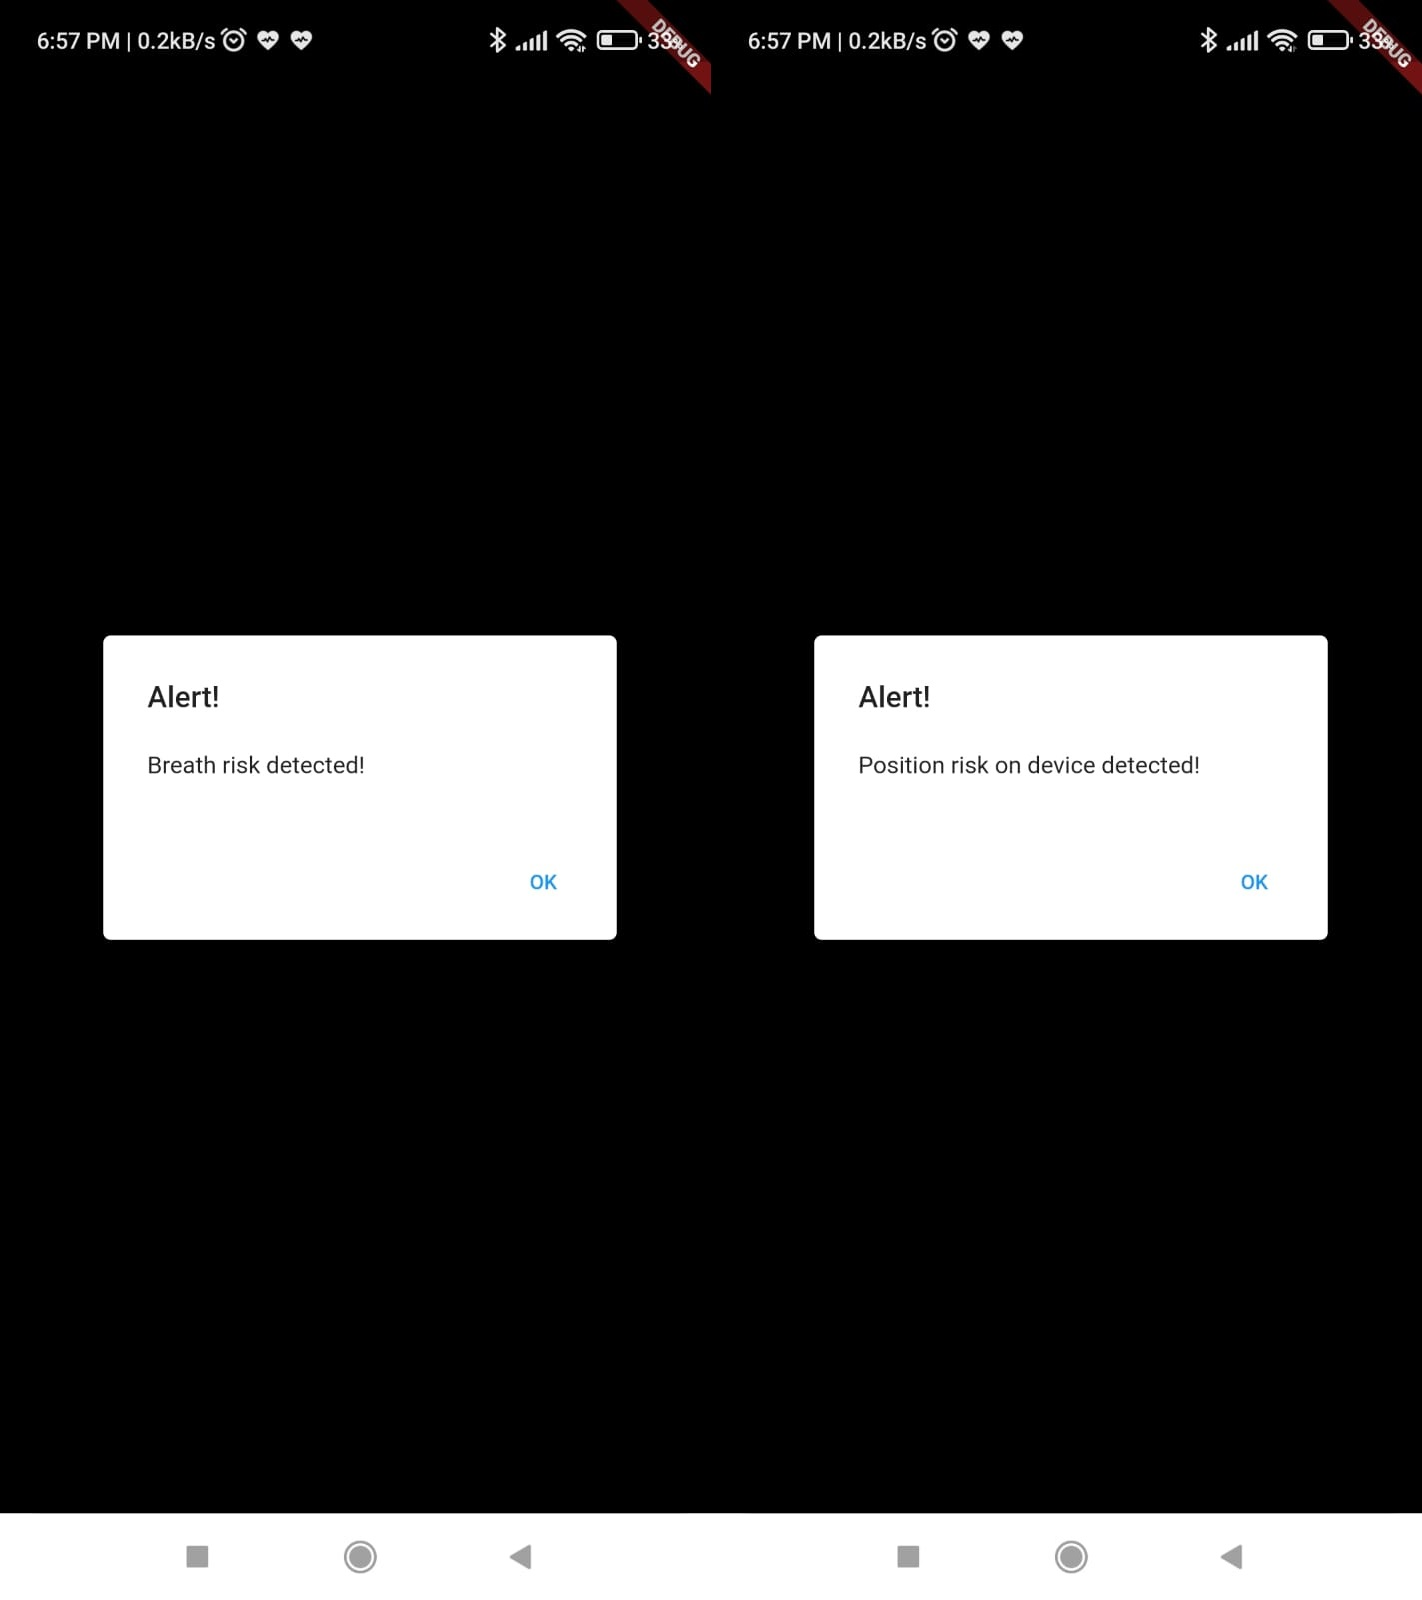
\includegraphics[width = 0.35 \textwidth]{risks.jpg}
            \caption{Pantallas de alerta.}
            \label{fig: risks_app}
        \end{figure}
        \FloatBarrier
        
    En la figura \ref{fig:risks_app} se muestran las alertas emitidas por la app cuando se presenta
    un posible riesgo, ests alertas tambien emiten sonido.

    \end{itemize}


